\documentclass[a4paper,11pt]{article}
\usepackage{amssymb}
\usepackage[polish]{babel}
\usepackage[utf8]{inputenc}
\usepackage[T1]{fontenc}
\usepackage{graphicx}
\usepackage{anysize}
\usepackage{enumerate}
\usepackage{times}
\usepackage{geometry}
\usepackage{amsthm}
\usepackage{pgfplots}

\usepackage[intlimits]{amsmath}
\marginsize{3cm}{3cm}{1.5cm}{1.5cm}
\sloppy

\begin{document}
\begin{table}[ht]
\centering
\hspace*{-1cm}
\begin{tabular}{lllllll}
\cline{1-6}
\multicolumn{1}{|c|}{\begin{tabular}[c]{@{}c@{}}EAIiIB\\ Informatyka\end{tabular}}              & \multicolumn{2}{l|}{\begin{tabular}[c]{@{}l@{}}Ewa Stachów\\ Weronika Olcha\end{tabular}}                                                                                                & \multicolumn{1}{c|}{\begin{tabular}[c]{@{}c@{}}Rok\\ II\end{tabular}}          & \multicolumn{1}{c|}{\begin{tabular}[c]{@{}c@{}}Grupa\\ 3\end{tabular}}            & \multicolumn{1}{c|}{\begin{tabular}[c]{@{}c@{}}Zespół\\ 6\end{tabular}}      &  \\ \cline{1-6}
\multicolumn{1}{|c|}{\begin{tabular}[c]{@{}c@{}}Pracownia\\ FIZYCZNA\\ WFiIS AGH\end{tabular}} & \multicolumn{4}{l|}{\begin{tabular}[c]{@{}l@{}}Temat:\\ \textbf{\textit{Elektroliza}} \end{tabular}}                                                                                                                                                                                                                                            & \multicolumn{1}{c|}{\begin{tabular}[c]{@{}c@{}}Nr ćwiczenia:\\ 35\end{tabular}} &  \\ \cline{1-6}
\multicolumn{1}{|l|}{\begin{tabular}[c]{@{}c@{}}Data wykonania:\\ 05.11.2016\end{tabular}}      & \multicolumn{1}{c|}{\begin{tabular}[c]{@{}c@{}}Data oddania:\\ 09.11.2016\end{tabular}} & \multicolumn{1}{l|}{\begin{tabular}[c]{@{}l@{}}Zwrot do poprawki:\\ \phantom{data poprawki}\end{tabular}} & \multicolumn{1}{l|}{\begin{tabular}[c]{@{}l@{}}Data oddania:\\  \phantom{data oddania}\end{tabular}} & \multicolumn{1}{l|}{\begin{tabular}[c]{@{}l@{}}Data zaliczenia:\\  \phantom{data zaliczenia}\end{tabular}} & \multicolumn{1}{l|}{\begin{tabular}[c]{@{}l@{}}OCENA:\\ \phantom{ocena}\end{tabular}}       &  \\ \cline{1-6}
                                                                                                
\end{tabular}
\end{table}

\begin{center}
\begin{LARGE}
\textbf{Ćwiczenie nr 35: Elektroliza}
\end{LARGE}
\end{center}

\section{Cel ćwiczenia}

Wyznaczanie równoważnika  elektrochemicznego    miedzi    oraz    stałej    Faradaya w doświadczeniu z~elektrolizą wodnego roztworu $\text{CuSO}_4$

\section{Wstęp teoretyczny}
Elektroliza zachodzi w układach, w których występują substancje zdolne do jonizacji, czyli rozpadu na jony. Samo zjawisko jonizacji może być wywołane zarówno przyłożonym napięciem elektrycznym, jak i zjawiskami nie generowanymi bezpośrednio przez prąd – dysocjacją elektrolityczną, autodysocjacją, wysoką temperaturą czy działaniem silnego promieniowania.

By zobojętnić jon na elektrodzie, musi przepłynąć ładunek równy $w\dot e$, gdzie $e$ - ładunek elementarny elektronu, a $w$ - wartościowość jonu.
Liczbę atomów które wydzieliły się na elektrodzie możemy wyznaczyć jako stosunek całkowitego ładunku ($I\dot t$) do ładunku pojedynczego jonu ($we$)
\begin{equation}
N=\frac{It}{we}
\end{equation}
Aby obliczyć masę osadzonych atomów, mnożymy ich ilość przez masę jednego atomu. Masę pojedynczego atomu można wyznaczyć jako stosunek masy molowej do
liczby Avogadra, stąd
\begin{equation}
\label{eq:masa}
m=N\frac{\mu}{N_A}=\frac{\mu}{weN_A}It
\end{equation}

Zauważamy, że masa wydzielonej substancji jest proporcjonalna do natężenia prądu $I$, czasu przepływu prądu $t$ oraz współczynnika oznaczanego $k$ i zwanego elektrochemicznym równoważnikiem substancji.
\begin{equation}
\label{eq:k}
k=\frac{\mu}{weN_A}
\end{equation}


Iloczyn $eN_A$ wyraża ładunek potrzebny do wydzielenie jednego gramorównoważnika chemicznego substancji. Oznacza się go zwykle jako $F$ i nazywa stałą Faradaya.
Ze wzoru (\ref{eq:k}) wynika jego zależność od $k$:
\begin{equation}
%\label{eq:k}
F=\frac{\mu}{wk}
\end{equation}

Nie należy mylić elektrolizy z procesami zachodzącymi w ogniwie galwanicznym. W elektrolizie energia elektryczna zamieniana jest na chemiczną, a w ogniwie galwanicznym kierunek przemian energetycznych jest przeciwny, tzn. energia chemiczna w procesie reakcji redoks zamieniana jest na energię elektryczną, co objawia się generowaniem prądu w obwodzie łączącym elektrody ogniwa. Ze względu na odwrotny przebieg procesu w ogniwach galwanicznych katoda jest naładowana dodatnio, a anoda ujemnie, jednak procesy chemiczne zachodzące na obu ogniwach mają podobny charakter.

\section{Układ pomiarowy}


\subsubsection*{Przyrządy}
\begin{itemize}
\item Naczynie do elektrolizy siarczanu miedzi $\text{CuSO}_4$ z miedzianymi elektrodami w kształcie
równoległych płyt, oddalonych od siebie o kilka centymetrów (rys. 1).
\item Zasilacz napięcia stałego
\item Amperomierz
\item Opornica suwakowa
\item Waga elektroniczna
\end{itemize}

\begin{figure}[h!]
\centering
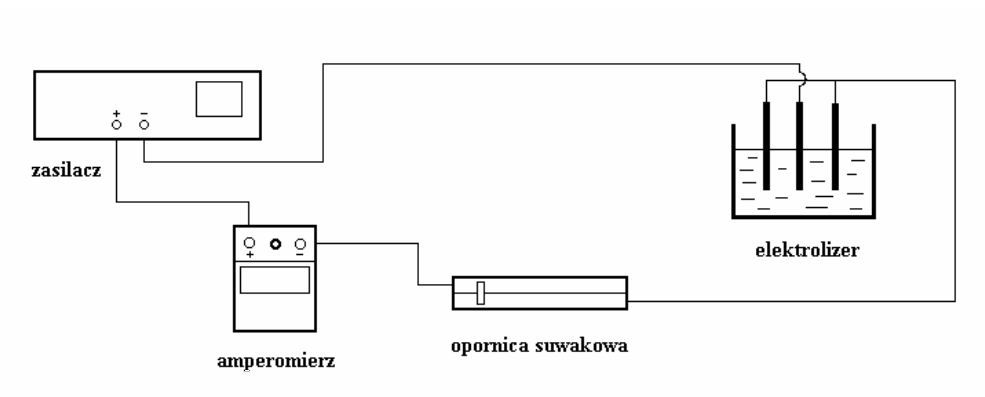
\includegraphics[width=0.7\linewidth]{./uklad}
\caption{Schemat obwodu elektrycznego}
\label{fig:uklad}
\end{figure}


\section{Wyniki pomiarów}
\begin{center}
\begin{tabular}{lrlll}
czas elektrolizy               & $t$ & = & 30 & min  \\ 
natężenie prądu               &  $I$ & = & 0,5 & A \\ 
masa katody przed elektrolizą &  $m_1$ & = & 93,828 & g \\ 
masa katody po elektrolizie  &   $m_2$ & = & 94,134 & g\\ 
masa wydzielonej miedzi       &  $m = m_2 - m_1$& = & 0,306 & g \\ 
masa anod przed elektrolizą   &   ${M_1}_{A}$ & = &126,699 & g\\ 
  &   ${M_1}_{B}$ & = &122,350 & g\\ 
masa anod po elektrolizie     &   ${M_2}_{A}$ & = &126,520 & g\\
  &   ${M_2}_{B}$ & = &122,213 & g\\  
zmiana masy anod               &  $M = M_2 - M_1$& = & 0,316 & g \\  
\end{tabular} 
\end{center}

\subsection*{Dane określające niepewność przyrządów:}
\begin{center}
\begin{tabular}{lrlll}
Klasa amperomierza              & &  & 0,5 &   \\ 
Używany zakres amperomierza               &   &  & 0,75 & A \\ 
Niepewność graniczna wagi (znamionowa)&  $\Delta m$ & = & 0,001 & g \\ 
Niepewność pomiaru masy &   $u(m)$& = & 0,00058 & g\\  
\end{tabular} 
\end{center}

\section{Opracowanie wyników}
Aby obliczyć współczynnik elektrochemiczny $k$ korzystamy ze wzoru:
$$
k = \frac{m}{I t} = \frac{0,306}{0,5 \cdot 30 \cdot 60} \frac{g}{A \cdot s}  = 0,340 \cdot 10^{-3} \frac{g}{A \cdot s} 
$$
Korzystając z otrzymanej wartości współczynnika  $k$ i  wzoru obliczamy doświadczalną wartość stałej Faradaya ze wzoru;
$$
F = \frac{\mu}{w k} = \frac{63,58 }{2 \cdot 0,340 \cdot 10^{-3}} \frac{C}{mol} = 93500~\frac{C}{mol}, 
$$
gdzie $\mu$ to masa molowa miedzi $63,5~\dfrac{g}{mol}$, a $w$ to wartościowość miedzi równa 2.

Korzystając z otrzymanej wartości stałej Faradaya  $F$, obliczamy doświadczalną wartość ładunku elementarnego :
$$
e = \frac{F}{N_A} = \frac{93500}{6,0222 \cdot 10^{23}}~C = 1,552 \cdot 10^{-19}~C,  
$$
gdzien $N_A$ to liczba Avogadra, która jest wielkością stałą informującą o liczbie cząsteczek lub atomów zawartych w jednym molu substancji. 
\section{Obliczanie niepewności pomiarowej}
Niepewność pomiaru czasu przyjmujemy $u(t)=5s$, ze względu na opóźnioną reakcję przy włączaniu stopera. 

Mimo, iż niepewność pomiaru wagi wynosiła 0,001g my przyjmujemy ją jako:
$$
u(m) = 0,005 g
$$
Związane jest to z możliwością niedokładnego wysuszenia elektrod, niedokładnego ich przepłukania lub zanieczyszczenia samego elektrolitu.

Aby policzyć niepewność wartości ładunku elektrycznego, który przepłynął przez elektrolit musimy znać niepewność pomiaru natężenia:
$$
u(I) = \frac{\text{klasa amperomierza} \cdot \text{zakres}}{100} = 3,75 \cdot 10^{-3}~A
$$
A zatem niepewność wartości ładunku elektrycznego wynosi:
$$
u(e) = t \cdot u(I) = 1800 \cdot 3,75 \cdot 10^{-3} ~C= 2,539 ~C
$$

\subsubsection*{Niepewność względna i bezwzględna  równoważnika elektrochemicznego}  

$$
\frac{u(k)}{k} = \sqrt{\left[\frac{u(m)}{m} \right]^2 + \left[\frac{u(I)}{I} \right]^2 } = \sqrt{\left[\frac{ 0,005}{0,306} \right]^2 + \left[\frac{0,00375}{0,5} \right]^2 } \approx 0,018
$$

$$
u(k) = \frac{u(k)}{k} \cdot k =  0,018 \cdot 0,340 \cdot 10^{-3} \approx 0,0061 \cdot 10^{-3} ~ \frac{g}{A \cdot s}
$$

\subsubsection*{Niepewność względna i bezwzględna  stałej Faradaya oraz ładunku elementarnego}

$$
\frac{u(F)}{F} = \sqrt{\left[\frac{u(\mu)}{\mu} \right]^2 + \left[\frac{u(k)}{k} \right]^2 } = \sqrt{\left[\frac{u(k)}{k} \right]^2 } = \frac{u(k)}{k}  =   \frac{u(e)}{e}
$$

$$
u(F) = F \frac{u(k)}{k}  =  96500  \cdot  0,018 = 1700,93  ~ \frac{C}{mol} 
$$

$$
u(e) = e \frac{u(k)}{k}  =  1,552 \cdot 10^{-19}  \cdot  0,018 = 0,028 \cdot 10^{-19} ~C 
$$

\section{Podsumowanie wyników}

\begin{tabular}{|l|p{2cm}|p{2,2cm}| p{2cm}| p{2cm} | p{2,2cm}|}
\hline  & wartość tablicowa  & wartość wyznaczona& różnica & niepewność  & niepewność względna [\%]  \\ 
\hline $k \left[  \frac{mg}{A \cdot s}\right]$ & 0,329  & 0,340  & 0,011 & 0,0061  & 1,8  \\ 
\hline $F \left[  \frac{C}{mol}\right]$ & 96500 & 93500  & 3000  & 1700,97  & 1,8  \\ 
\hline $e [10^{-19} C]$ & 1,602   & 1,552    & 0,05    & 0,028   & 1,8  \\ 
\hline 
\end{tabular} 

\section{Wnioski}
\begin{itemize}

\item Masa anod uległa zmniejszeniu, a masa katody zwiększeniu. 
\item Wyznaczone wielkości stałej Faradaya, równoważnika elektrochemicznego miedzi oraz ładunku elementarnego nie mieszczą się w granicach błędu. Wyjaśnia to zapewne możliwość powstanie sporego błędu przypadkowego, jak np. niedokładne wysuszenie płytek, niedokładne ich opłukanie lub zanieczyszczenie elektrolitu. 
\item Elektrolity mogą być dobrymi przewodnikami. 
 
\end{itemize}

\end{document}